\chapter{Unity DOTS: Sviluppo del Prototipo}
\label{cap:prototipo}

Al fine di fornire una dimostrazione pratica dell'utilizzo dell'architettura Unity DOTS, abbiamo realizzato il seguente prototipo, che consiste in un piccolo gioco multigiocatore. L'obbiettivo del progetto è quello di realizzare un gameplay basilare, con movimento dei personaggi e piccole interazioni con l'ambiente di gioco, ad esempio la raccolta degli oggetti di scena. In particolare, ogni giocatore controlla il proprio ``CapsulePlayer'' e può interagire con gli oggetti di scena grazie al sistema di collisione e trigger fornito dal package Physics. La trattazione di quest'ultimo esula dall'argomento della tesi, per cui si rimanda alla documentazione ufficiale disponibile a~\cite{doc:unity-physics-manual}.

\begin{figure}[!ht]
    \centering
    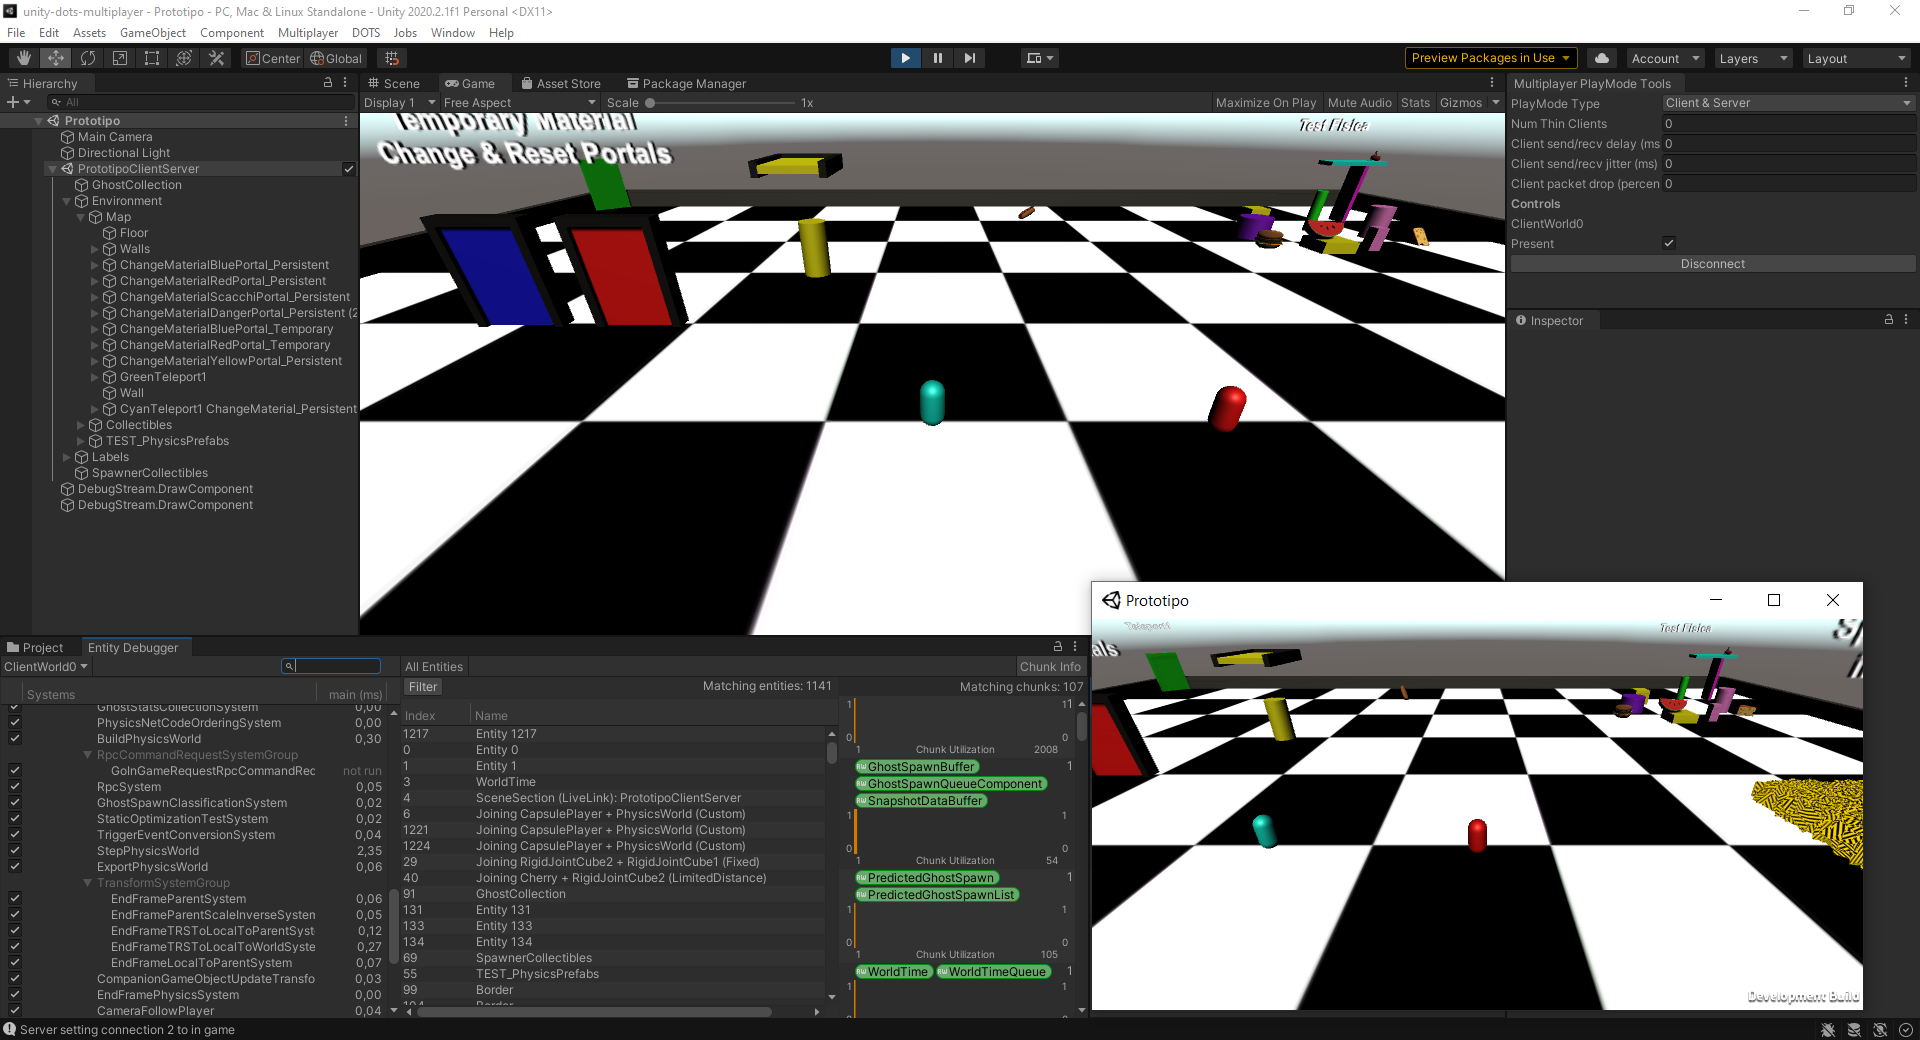
\includegraphics[width=0.95\columnwidth]{gfx/imgs/chapter4/ShowcasePrototipo.png}
    \caption{Prototipo Unity DOTS.}
    \label{fig:prototipo-dots}
\end{figure}

\section{Funzionalità}
Il prototipo permette di avviare un server in ascolto sulla porta 7979, e al quale i client possono connettersi. Una volta stabilita la connessione, il server fa entrare in gioco i client e per ciascuno di essi crea un personaggio capsula all'interno della scena. Da questo momento i vari giocatori possono iniziare a muoversi all'interno della mappa di gioco, interagendo con i molteplici oggetti di scena. In particolare, sono presenti:

\begin{itemize}
    \item Portali che cambiano il materiale di ciò che li attraversa in modo temporaneo o permanente.
    \item Teletrasporti.
    \item Oggetti di varie forme, dimensioni e proprietà fisiche.
    \item Oggetti raccoglibili e che incrementano il punteggio del giocatore.
\end{itemize}

\section{Sviluppo e implementazione}

Il prototipo è stato realizzato utilizzando Unity2020.2.1f1. Abbiamo creato un progetto 3D vuoto e, oltre ai package di default di Unity, vi abbiamo aggiunto i seguenti package: \textbf{Entities}, Hybrid Renderer, Platform Windows, \textbf{NetCode}, Transport, Physics.

\begin{figure}[!ht]
    \begin{subfigure}{.49\textwidth}
      \centering
      % include first image
      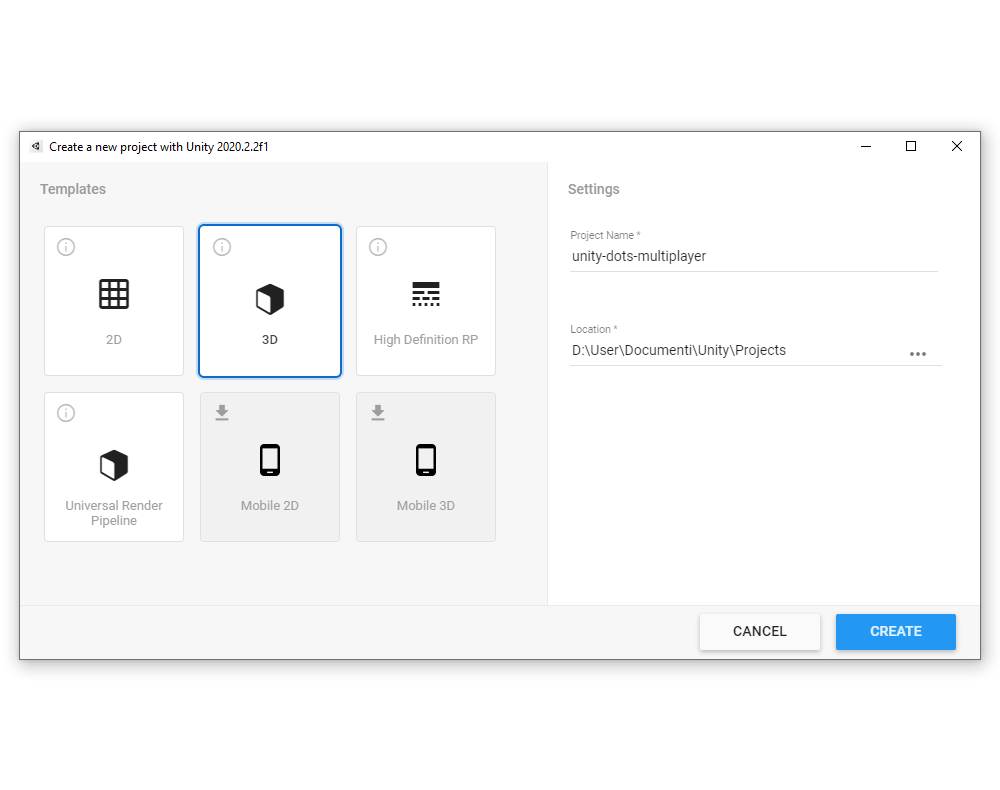
\includegraphics[width=.95\linewidth]{gfx/imgs/chapter4/CreazioneProgetto.png}
      \caption{Creazione progetto.}
      \label{fig:prototipo-creazione-progetto}
    \end{subfigure}
    \begin{subfigure}{.49\textwidth}
      \centering
      % include second image
      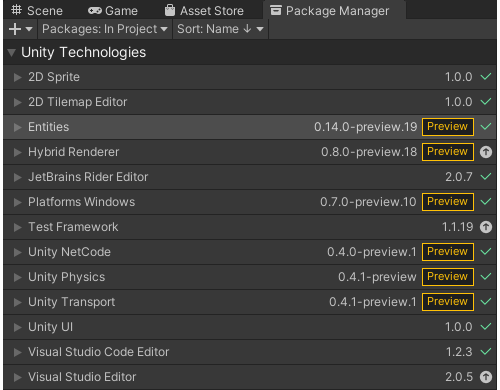
\includegraphics[width=.95\linewidth]{gfx/imgs/chapter4/PackagesPrototipo(actual)2.png}
      \caption{Package Manager.}
      \label{fig:prototipo-packages}
    \end{subfigure}
    \caption{Creazione del progetto e setup.}
    \label{fig:prototipo-setup-progetto}
\end{figure}

Al momento della creazione del prototipo, la maggior parte di questi package vengono forniti attraverso una versione di preview. Di conseguenza, per importarli è stato necessario aprire il pannello \emph{Package Manager} (Figura~\ref{fig:prototipo-packages}) ed inserire l'URL di ognuno dei package manualmente. (Figura~\ref{fig:prototipo-import-packages}). Per ottenere l'URL specifico del package che vogliamo importare, possiamo fare riferimento al manuale ufficiale di Unity~\cite{doc:unity-preview-packages}.


\begin{figure}[!ht]
    \begin{subfigure}{.49\textwidth}
      \centering
      % include first image
      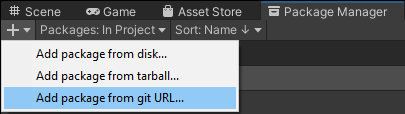
\includegraphics[width=.95\linewidth]{gfx/imgs/chapter4/SetupAddPackageFromURL.png}
      \caption{Aggiunta package tramite URL.}
      \label{fig:prototipo-import1}
    \end{subfigure}
    \begin{subfigure}{.49\textwidth}
      \centering
      % include second image
      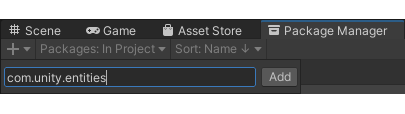
\includegraphics[width=.95\linewidth]{gfx/imgs/chapter4/SetupAddPackageFromURL(2).png}
      \caption{Esempio aggiunta di Entities.}
      \label{fig:prototipo-import2}
    \end{subfigure}
    \caption{Importazione package nel progetto.}
    \label{fig:prototipo-import-packages}
\end{figure}

In alternativa è possibile importare i package aggiungendo gli URL e la relativa versione che si desidera utilizzare, nel file manifest.json, che si trova nella sottodirectory Packages del progetto.

\subsection{Connessione}

Per avviare il gioco possiamo entrare in Play Mode dall'editor Unity, oppure possiamo lanciare una build standalone. Fatto ciò, entra in esecuzione il sistema \verb|Game|. Questo sistema si occupa di stabilire la connessione tra i vari client ed il server; e tramite la chiamata al metodo \verb|RequireSingletonForUpdate| ed il componente \verb|InitGameComponent|, ci assicuriamo che il sistema esegua una sola volta per ogni avvio dell'applicazione.

All'interno di \verb|OnUpdate()| il sistema elimina il componente singleton \verb|InitGameComponent| ed itera su tutti i mondi disponibili (vedi Codice~\ref{lst:prototipo-game-connessione}). Se all'interno di questi è presente il sistema \verb|ClientSimulationSystemGroup| significa che sta eseguendo un client, mentre se vi è \verb|ServerSimulationSystemGroup|, ci si trova nel server. Una volta ottenuto il sistema \verb|NetworkStreamReceiveSystem|, è possibile utilizzarne la classe per mettersi in ascolto delle connessioni su qualsiasi indirizzo (nel nostro caso sulla porta 7979), qualora ci si trovi nel server, oppure connettersi a quest'ultimo nel caso del client.
\SaveVerb{GameTerm}|Game.cs|

\begin{lstlisting}[caption={File \UseVerb{GameTerm}: stabilimento della connessione.}, label={lst:prototipo-game-connessione}, language={[Sharp]C}]
public struct EnableGame : IComponentData
{
}

[UpdateInWorld(UpdateInWorld.TargetWorld.Default)]
[AlwaysSynchronizeSystem]
public class Game : SystemBase
{
    struct InitGameComponent : IComponentData
    {
    }
    protected override void OnCreate()
    {
        RequireSingletonForUpdate<InitGameComponent>();
        EntityManager.CreateEntity(typeof(InitGameComponent));
    }
    protected override void OnUpdate()
    {
        EntityManager.DestroyEntity(GetSingletonEntity<InitGameComponent>());
        foreach (var world in World.All)
        {
            var network = world.GetExistingSystem<NetworkStreamReceiveSystem>();
            if (world.GetExistingSystem<ClientSimulationSystemGroup>() != null)
            {
                world.EntityManager.CreateEntity(typeof(EnableGame));
                NetworkEndPoint ep = NetworkEndPoint.LoopbackIpv4;
                ep.Port = 7979;
                network.Connect(ep); // connect a localhost:7979
            }
            else if (world.GetExistingSystem<ServerSimulationSystemGroup>() != null)
            {
                world.EntityManager.CreateEntity(typeof(EnableGame));
                NetworkEndPoint ep = NetworkEndPoint.AnyIpv4;
                ep.Port = 7979;
                network.Listen(ep);
            }
        }
    }
}
\end{lstlisting}

A questo punto client e server sono connessi. Ora è necessario implementare la logica che permette ai client di entrare in gioco e creare i rispettivi personaggi capsula.
Abbiamo implementato questa meccanica tramite la RPC \verb|GoInGameRequest|: il sistema \verb|GoInGameClientSystem| esegue solo se alla connessione non sia ancora stato associato il componente \verb|NetworkStreamInGame|. In tal caso, iteriamo sulle entità associate ad un \verb|NetworkIdComponent|, ovvero il componente che rappresenta una connessione. Infatti, come spiegato nella Sezione~\ref{subsec:netcode-stabilire-connessione}, per avviare la comunicazione dev'essere presente il componente \verb|NetworkStreamInGame|. In questo modo, il client può iniziare a inviare comandi e ricevere snapshot dal server. Nel caso \verb|NetworkStreamInGame| non sia presente, il sistema \verb|GoInGameClientSystem| invia una richiesta RPC al server, creando un'entità e aggiungendovi i componenti \verb|GoInGameRequest| e \verb|SendRpcCommandRequestComponent|. 

\begin{lstlisting}[caption={File \UseVerb{GameTerm}: richiesta di ingresso in gioco del client.}, label={lst:prototipo-game-start-client}, language={[Sharp]C}]
public struct GoInGameRequest : IRpcCommand
{
}

[UpdateInGroup(typeof(ClientSimulationSystemGroup))]
[AlwaysSynchronizeSystem]
public class GoInGameClientSystem : SystemBase
{
    protected override void OnCreate()
    {
        RequireSingletonForUpdate<EnableGame>();
        RequireForUpdate(GetEntityQuery(ComponentType.ReadOnly<NetworkIdComponent>(),
            ComponentType.Exclude<NetworkStreamInGame>()));
    }
    protected override void OnUpdate()
    {
        var commandBuffer = new EntityCommandBuffer(Allocator.Temp);
        Entities
            .WithNone<NetworkStreamInGame>()
            .ForEach((Entity ent, in NetworkIdComponent id) =>
        {
            commandBuffer.AddComponent<NetworkStreamInGame>(ent);
            var req = commandBuffer.CreateEntity();
            commandBuffer.AddComponent<GoInGameRequest>(req);
            commandBuffer.AddComponent(req, 
                new SendRpcCommandRequestComponent { TargetConnection = ent });
        }).Run();
        commandBuffer.Playback(EntityManager);
        commandBuffer.Dispose();
    }
}
\end{lstlisting}

Lato server, eseguiamo il sistema \verb|GoInGameServerSystem|, il quale si aggiorna solo quando viene rilevata la ricezione di una RPC di tipo \verb|GoInGameRequest|. 

Innanzitutto, il server ottiene un  \verb|GhostPrefabCollectionComponent|, in cui troviamo il prefab della capsula da creare per il giocatore. Come possiamo notare da Codice~\ref{lst:prototipo-game-start-server}, il sistema itera sulla lista dei ghost e prende solo quello con il componente \verb|PlayerMovementSpeed|, ovvero \verb|CapsulePlayer|. A questo punto, iteriamo su tutte le entità che hanno il componente \verb|GoInGameRequest| (la nostra RPC) e \verb|ReceiveRpcCommandRequestComponent|. In questo modo, possiamo ottenere la connessione del client che ha inviato tale richiesta. Così facendo, possiamo non solo far entrare un giocatore in gioco quando viene ricevuta la RPC, ma riusciamo anche ad assegnare al ghost \verb|CapsulePlayer| del client il \verb|NetworkId| relativo. Questo è molto importante perché è ciò che ci permette di distinguere le varie capsule dei giocatori a runtime. Infatti, l'assegnazione del \verb|NetworkId| deve necessariamente avvenire tramite il codice, in quanto a compile time ancora non si conosce a chi apparterrà una certa capsula.

A tal proposito, per realizzare le operazioni relative alla ricezione della RPC, abbiamo sfruttato un \verb|EntityCommandBuffer| (Codice~\ref{lst:prototipo-game-start-server}). In particolare, i passi che dobbiamo eseguire sono:
\begin{enumerate}
    \item Aggiungere il componente \verb|NetworkStreamInGame| alla connessione.
    \item Creare la capsula del giocatore.
    \item Inizializzare il \verb|NetworkId| della capsula del client a cui appartiene.
    \item Aggiungere il buffer \verb|PlayerInput| (che servirà in seguito per accumulare i comandi del giocatore).
    \item Infine, dobbiamo eliminare l'entità relativa alla RPC, altrimenti il \verb|ForEach| eseguirebbe di nuovo.
\end{enumerate}

\begin{lstlisting}[caption={File \UseVerb{GameTerm}: ricezione della RPC e avvio della comunicazione con il server, tramite stream di comandi e snapshot.}, label={lst:prototipo-game-start-server}, language={[Sharp]C}]
[UpdateInGroup(typeof(ServerSimulationSystemGroup))]
[AlwaysSynchronizeSystem]
public class GoInGameServerSystem : SystemBase
{
    protected override void OnCreate()
    {
        RequireSingletonForUpdate<EnableGame>();
        RequireForUpdate(GetEntityQuery(ComponentType.ReadOnly<GoInGameRequest>(), ComponentType.ReadOnly<ReceiveRpcCommandRequestComponent>()));
    }
    protected override void OnUpdate()
    {
        var ghostCollection = GetSingletonEntity<GhostPrefabCollectionComponent>();
        var prefab = Entity.Null;
        var prefabs = EntityManager.GetBuffer<GhostPrefabBuffer>(ghostCollection);
        for (int ghostId = 0; ghostId < prefabs.Length; ++ghostId)
        {
            if (EntityManager.HasComponent<PlayerMovementSpeed>(
                prefabs[ghostId].Value))
                prefab = prefabs[ghostId].Value;
        }

        var commandBuffer = new EntityCommandBuffer(Allocator.Temp);
        var networkIdFromEntity = GetComponentDataFromEntity<NetworkIdComponent>(true);
        Entities
            .WithReadOnly(networkIdFromEntity)
            .ForEach((Entity reqEnt, in GoInGameRequest req, 
                in ReceiveRpcCommandRequestComponent reqSrc) =>
        {
            // da qui in poi sara' possibile inviare comandi e ricevere snapshot
            commandBuffer.AddComponent<NetworkStreamInGame>(reqSrc.SourceConnection);
            UnityEngine.Debug.Log(String.Format("Server setting connection {0} to in game", networkIdFromEntity[reqSrc.SourceConnection].Value));

			// spawn della capsula e aggiornamento dell'ID del ghost
            var player = commandBuffer.Instantiate(prefab);
            commandBuffer.SetComponent(player, new GhostOwnerComponent { 
                NetworkId = networkIdFromEntity[reqSrc.SourceConnection].Value });

            commandBuffer.AddBuffer<PlayerInput>(player);
            commandBuffer.SetComponent(reqSrc.SourceConnection, 
                new CommandTargetComponent { targetEntity = player });

            commandBuffer.DestroyEntity(reqEnt);
        }).Run();
        commandBuffer.Playback(EntityManager);
        commandBuffer.Dispose();
    }
}
\end{lstlisting}

Per far sì che questo funzioni, come spiegato nella Sezione~\ref{subsubsec:comunicazione-rpc}, nei mondi di client e server esegue il sistema \verb|RpcSystem|. Questo si occupa della serializzazione e deserializzazione delle RPC. Inoltre, il \verb|RpcSystem| svolge due importanti funzioni: lato mittente elimina l'entità relativa alla RPC, mentre lato destinatario aggiunge il componente \verb|ReceiveRpcCommandRequestComponent|.

\begin{figure}[!ht]
    \begin{subfigure}{.54\textwidth}
      \centering
      % include first image
      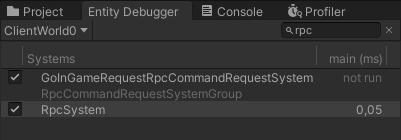
\includegraphics[width=.95\linewidth]{gfx/imgs/chapter4/RpcSystemClient.png}
      \caption{Client.}
      \label{fig:rpc-system-client}
    \end{subfigure}
    \begin{subfigure}{.45\textwidth}
      \centering
      % include second image
      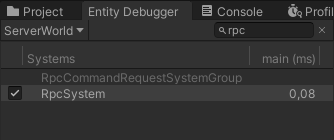
\includegraphics[width=.95\linewidth]{gfx/imgs/chapter4/RpcSystemServer.png}
      \caption{Server.}
      \label{fig:rpc-system-server}
    \end{subfigure}
    \caption{RpcSystem in esecuzione su client e server.}
    \label{fig:rpc-system}
\end{figure}

\subsection{Comunicazione}
Ora che le connessioni sono state marcate come ``in gioco'', client e server possono comunicare tramite stream di comandi e snapshot. In particolare, il client invia i comandi relativi al movimento della propria capsula, ed il server manda continuamente uno stream di snapshot riguardo lo stato di gioco dei vari ghost.

\subsubsection{Input giocatore}

\SaveVerb{CommandTargetComponentTerm}|CommandTargetComponent|
Come spiegato nel Capitolo~\ref{cap:netcode}, per poter inviare dei comandi è necessario creare una struttura di tipo \verb|ICommandData|, che implementa la proprietà \verb|Tick|. Nel nostro caso (Codice~\ref{lst:prototipo-input-client}) \verb|PlayerInput| contiene i campi \verb|horizontal| e \verb|vertical|. Questi ultimi rappresentano il segno che assumerà il valore della velocità della capsula sugli assi X e Z.

Lato client, la raccolta degli input del giocatore avviene tramite il sistema \verb|PlayerInputSystem|. All'interno di questo sistema, nel metodo \verb|OnUpdate()|, come prima cosa verifichiamo che il singleton \verb|CommandTargetComponent|\footnote{\UseVerb{CommandTargetComponentTerm} è un singleton, diverso per ogni client, che contiene il riferimento all'entità su cui verranno applicati i comandi, ovvero l'unica appartenente al giocatore. Nel nostro caso è la capsula.} contenga il riferimento all'entità associata alla capsula. 
Se il riferimento risulta essere nullo, significa che ci troviamo nella prima esecuzione del sistema. Di conseguenza, dobbiamo semplicemente trovare la capsula che corrisponde al \verb|NetworkId| del giocatore e associarla a \verb|CommandTargetComponent|, perché sicuramente è già stata creata in Codice~\ref{lst:prototipo-game-start-server}.

Dunque, per trovare la nostra capsula iteriamo su tutte le entità che hanno il componente \verb|PlayerMovementSpeed|, ovvero il componente tipico di \verb|CapsulePlayer|. Nei parametri della lambda expression aggiungiamo anche \verb|GhostOwnerComponent|, in quanto contiene il \verb|NetworkId| della capsula, che possiamo usare per ottenere quella appartenente al nostro client. Infatti, confrontando \verb|NetowrkId| con \verb|localPlayerId|, ottenuto dalla connessione, siamo sicuri che la capsula sia quella giusta e possiamo aggiungervi il buffer di comandi.

Una volta certi che \verb|CommandTargetComponent| contenga il riferimento alla capsula del client, possiamo iniziare a campionare gli input del giocatore. Per ogni comando da inviare al server è necessario aggiornare la proprietà \verb|Tick| di \verb|PlayerInput|. In questo modo, quando il server riceverà il comando, saprà a quale tick della sua simulazione applicarlo, per far sì che l'azione avvenga nello stesso momento di quella del client.\\

\SaveVerb{PlayerInputSystemTerm}|PlayerInputSystem.cs|

\begin{lstlisting}[caption={File \UseVerb{PlayerInputSystemTerm}: campionamento degli input del giocatore ed invio al server tramite stream di comandi bufferizzato.}, label={lst:prototipo-input-client}, language={[Sharp]C}]
public struct PlayerInput : ICommandData
{
    public uint Tick { get; set; }
    public int horizontal;
    public int vertical;
}

[UpdateInGroup(typeof(ClientSimulationSystemGroup))]
[AlwaysSynchronizeSystem]
public class PlayerInputSystem : SystemBase
{
    ClientSimulationSystemGroup m_ClientSimulationSystemGroup;
    protected override void OnCreate()
    {
        RequireSingletonForUpdate<NetworkIdComponent>();
        RequireSingletonForUpdate<EnableGame>();
        m_ClientSimulationSystemGroup =
            World.GetExistingSystem<ClientSimulationSystemGroup>();
    }

    protected override void OnUpdate()
    {
        var localInput = GetSingleton<CommandTargetComponent>().targetEntity;
        
		if (localInput == Entity.Null) // riferimento alla capsula assente
        {
			var localPlayerId = GetSingleton<NetworkIdComponent>().Value;
            var commandBuffer = new EntityCommandBuffer(Allocator.Temp);
            var commandTargetEntity = GetSingletonEntity<CommandTargetComponent>();
            
			Entities
			    .WithAll<PlayerMovementSpeed>()
			    .WithNone<PlayerInput>()
			    .ForEach((Entity ent, ref GhostOwnerComponent ghostOwner) =>
            {
				if (ghostOwner.NetworkId == localPlayerId)
                {
                    commandBuffer.AddBuffer<PlayerInput>(ent);
                    commandBuffer.SetComponent(commandTargetEntity, 
                        new CommandTargetComponent { targetEntity = ent });
                }
            }).Run();
            commandBuffer.Playback(EntityManager);
            return;
        }
        
		var input = default(PlayerInput);
		input.Tick = m_ClientSimulationSystemGroup.ServerTick;
        if (Input.GetKey("a"))
            input.horizontal -= 1;
        if (Input.GetKey("d"))
            input.horizontal += 1;
        if (Input.GetKey("s"))
            input.vertical -= 1;
        if (Input.GetKey("w"))
            input.vertical += 1;
        
        var inputBuffer = EntityManager.GetBuffer<PlayerInput>(localInput);
        inputBuffer.AddCommandData(input);
    }
}
\end{lstlisting}

\subsubsection{Movimento capsula}
Una volta che abbiamo campionato gli input possiamo applicarli alla capsula del giocatore. Il sistema che si occupa di questo meccanismo è chiamato  \verb|PlayerMovementSystem|. Possiamo notare come questo esegua all'interno del gruppo \verb|GhostPredictionSystemGroup|, il quale permette di implementare la predizione lato client dei ghost. In particolare, da questo gruppo otteniamo il \verb|PredictionTick|, che possiamo usare per sapere se è necessario eseguire la predizione. In caso negativo viene semplicemente terminata la funzione. Al contrario, in caso affermativo, traduciamo l'input campionato in un movimento. In particolare, aggiorniamo il valore della velocità della capsula e utilizziamo ancora una volta \verb|PredictionTick| per sapere a quale tick è necessario applicarlo.

\SaveVerb{PlayerMovementSystemTerm}|PlayerMovementSystem.cs|

\clearpage
\begin{lstlisting}[caption={File \UseVerb{PlayerMovementSystemTerm}: applicazione del movimento alla capsula, tramite predizione.}, label={lst:prototipo-input-server}, language={[Sharp]C}]
[UpdateInGroup(typeof(GhostPredictionSystemGroup))]
public class PlayerMovementSystem : SystemBase
{
    GhostPredictionSystemGroup m_GhostPredictionSystemGroup;
    protected override void OnCreate()
    {
        m_GhostPredictionSystemGroup =
            World.GetExistingSystem<GhostPredictionSystemGroup>();
    }
    #region Codice Predizione
    
    protected override void OnUpdate() 
    {
        var tick = m_GhostPredictionSystemGroup.PredictingTick;
        var deltaTime = Time.DeltaTime;
        Entities.ForEach((DynamicBuffer<PlayerInput> inputBuffer, 
            ref PhysicsVelocity pv, 
            in PredictedGhostComponent prediction, in PlayerMovementSpeed pms) =>
        {
            if (!GhostPredictionSystemGroup.ShouldPredict(tick, prediction))
                return;
            PlayerInput input;
            inputBuffer.GetDataAtTick(tick, out input);
            var speed = pms.speed;
            
            if (input.horizontal > 0)
                pv.Linear.x += speed * deltaTime;
            if (input.horizontal < 0)
                pv.Linear.x -= speed * deltaTime;
            if (input.vertical > 0)
                pv.Linear.z += speed * deltaTime;
            if (input.vertical < 0)
                pv.Linear.z -= speed * deltaTime;

        }).ScheduleParallel();
    }
    
    #endregion
}
\end{lstlisting}

\subsection{Azioni di gioco}
Oltre al semplice movimento, per rendere il prototipo un po' più interessante, abbiamo realizzato qualche funzionalità aggiuntiva, fra cui la raccolta degli oggetti e qualche portale interattivo.

\subsubsection{Raccolta oggetti}

Per realizzare la meccanica della raccolta degli oggetti, abbiamo innanzitutto creato un componente \verb|CollectibleTagComponent| per marcare le entità che possono essere raccolte.
Dopodiché, sfruttando il package \emph{Physics}, abbiamo implementato un sistema \verb|PickUpSystem| in grado di rilevare le collisioni tra l'entità dell'oggetto e quella di \verb|CapsulePlayer|. Il sistema, appena rileva il trigger della collisione, aggiorna il punteggio del giocatore e aggiunge il componente vuoto \verb|DeleteTagComponent| all'entità dell'oggetto raccoglibile.\\

\begin{lstlisting}[caption={Componente che marca un'entità come raccoglibile.}, label={lst:prototipo-collectible}, language={[Sharp]C}]
[GenerateAuthoringComponent]
public struct CollectibleTagComponent : IComponentData
{
    public float points;
}
\end{lstlisting}

\SaveVerb{PickUpSystemTerm}|PickUpSystem.cs|
\SaveVerb{DeleteTagComponentTerm}|DeleteTagComponent|

\begin{lstlisting}[caption={File \UseVerb{PickUpSystemTerm}: aumento del punteggio del giocatore e aggiunta del tag \UseVerb{DeleteTagComponentTerm} agli oggetti raccoglibili.}, label={lst:prototipo-pickup}, language={[Sharp]C}]
#region Pickup

Entities
    .WithoutBurst()
    .ForEach((Entity e, ref DynamicBuffer<StatefulTriggerEvent> triggerEventBuffer,
        ref CollectibleTagComponent collectibleComponent) =>
{
    for (int i = 0; i < triggerEventBuffer.Length; i++)
    {
        var triggerEvent = triggerEventBuffer[i]; // entita' A
        var otherEntity = triggerEvent.GetOtherEntity(e); // entita' B
        
        // [...]
        
        // quando entra nella hitbox
        if (triggerEvent.State == EventOverlapState.Enter && EntityManager.HasComponent<PlayerMovementSpeed>(otherEntity))
        {
            var punteggioPlayer =
                EntityManager.GetComponentData<PlayerScoreComponent>(otherEntity);
            punteggioPlayer.score += collectibleComponent.points;

            var ghostId =
                EntityManager.GetComponentData<GhostComponent>(otherEntity).ghostId;
            UnityEngine.Debug.Log(String.Format("Il player " + ghostId + 
                " ha raccolto " + collectibleComponent.points + " punti. Tot 
                punti player " + ghostId + ": " + punteggioPlayer.score));

            commandBuffer.SetComponent(otherEntity, punteggioPlayer);
            commandBuffer.AddComponent<DeleteTagComponent>(e, deleteTag);
        }
    }
}).Run();

#endregion
\end{lstlisting}

Il componente \verb|DeleteTagComponent| è un espediente che ci serve per eliminare gli oggetti raccolti: tramite il sistema \verb|DeleteCollectibleSystem| possiamo iterare su tutte le entità marcate da questo componente e rimuoverle.

\begin{lstlisting}[caption={Componente che marca un'entità come ``da eliminare''.}, label={lst:prototipo-delete-tag}, language={[Sharp]C}]
public struct DeleteTagComponent : IComponentData
{
}
\end{lstlisting}

\SaveVerb{DeleteCollectibleSystemTerm}|DeleteCollectibleSystem.cs|
\SaveVerb{DeleteTagComponentTerm}|DeleteTagComponent|

\begin{lstlisting}[caption={File \UseVerb{DeleteCollectibleSystemTerm}: eliminazione delle entità aventi il componente \UseVerb{DeleteTagComponentTerm}.}, label={lst:prototipo-delete-system}, language={[Sharp]C}]
[UpdateInGroup(typeof(ClientAndServerSimulationSystemGroup))]
public class DeleteCollectibleSystem : SystemBase
{
    protected override void OnUpdate()
    {
        EntityCommandBuffer commandBuffer =
            new EntityCommandBuffer(Unity.Collections.Allocator.Temp);

        Entities
            .WithAll<DeleteTagComponent>()
            .ForEach((Entity entity) =>
            {
                commandBuffer.DestroyEntity(entity);
            }).Run();

        commandBuffer.Playback(EntityManager);
        commandBuffer.Dispose();
    }
}
\end{lstlisting}

\begin{figure}[!ht]
    \begin{subfigure}{.49\textwidth}
      \centering
      % include first image
      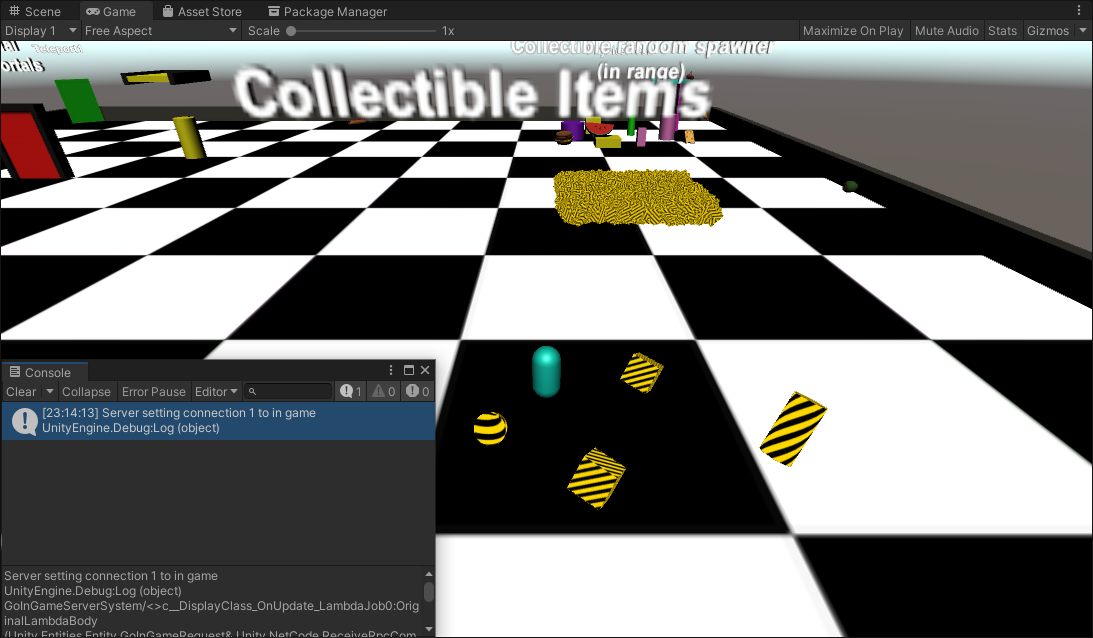
\includegraphics[width=.95\linewidth]{gfx/imgs/chapter4/PickUpCollectible1.png}
      \caption{Prima della raccolta dell'oggetto.}
      \label{fig:pickup-1}
    \end{subfigure}
    \begin{subfigure}{.49\textwidth}
      \centering
      % include second image
      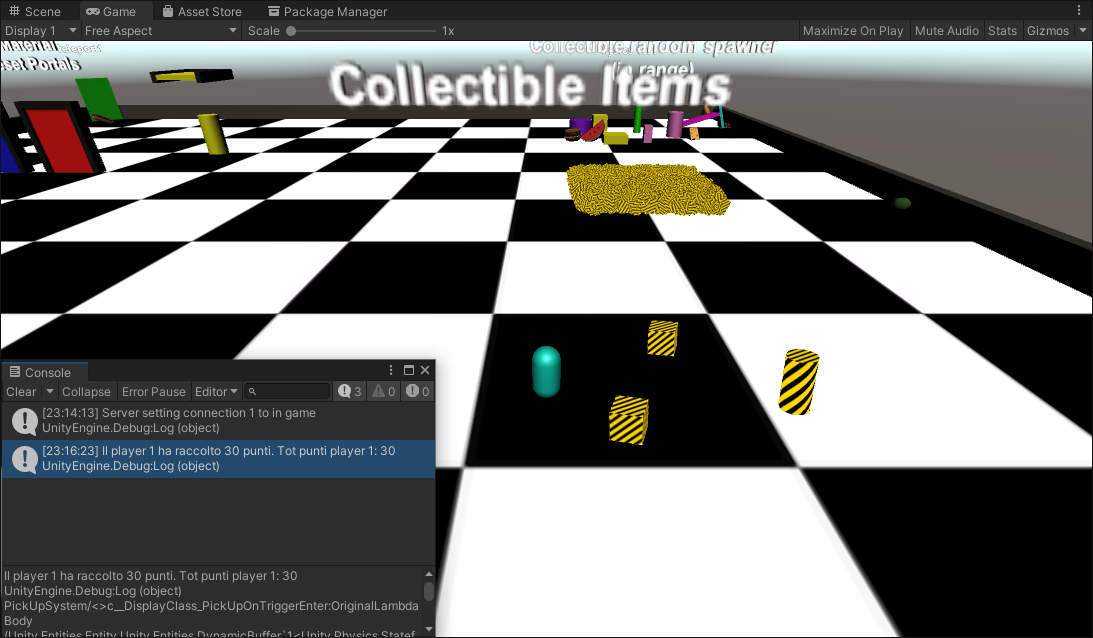
\includegraphics[width=.95\linewidth]{gfx/imgs/chapter4/PickUpCollectible2.png}
      \caption{Dopo la raccolta dell'oggetto.}
      \label{fig:pickup-2}
    \end{subfigure}
    \caption{Raccolta di un oggetto ``Sphere'' e stampa del log del punteggio.}
    \label{fig:pickup-collectibles}
\end{figure}

\subsubsection{Portali cambia-colore}

I portali sono stati realizzati sfruttando lo stesso meccanismo di \verb|PickUpSystem|:
il sistema \verb|PersistentChangeMaterialOnTriggerSystemTerm|, quando rileva il trigger di un'entità che lo attraversa, ne modifica il materiale con quello del portale stesso.

\SaveVerb{PersistentChangeMaterialOnTriggerSystemTerm}|PersistentChangeMaterialOnTriggerSystem.cs|
\SaveVerb{materialTerm}|material|

\begin{lstlisting}[caption={File \UseVerb{PersistentChangeMaterialOnTriggerSystemTerm}: aggiornamento del valore della proprietà \UseVerb{materialTerm} con quello del portale.}, label={lst:prototipo-portal-material}, language={[Sharp]C}]
#region Portale cambia colore

if (triggerEvent.State == EventOverlapState.Enter)
{
    var volumeRenderMesh = EntityManager.GetSharedComponentData<RenderMesh>(e);
    var overlappingRenderMesh = EntityManager.GetSharedComponentData<RenderMesh>(otherEntity);
    overlappingRenderMesh.material = volumeRenderMesh.material;

    commandBuffer.SetSharedComponent(otherEntity, overlappingRenderMesh);
}

#endregion
\end{lstlisting}

\begin{figure}[!ht]
    \begin{subfigure}{.49\textwidth}
      \centering
      % include first image
      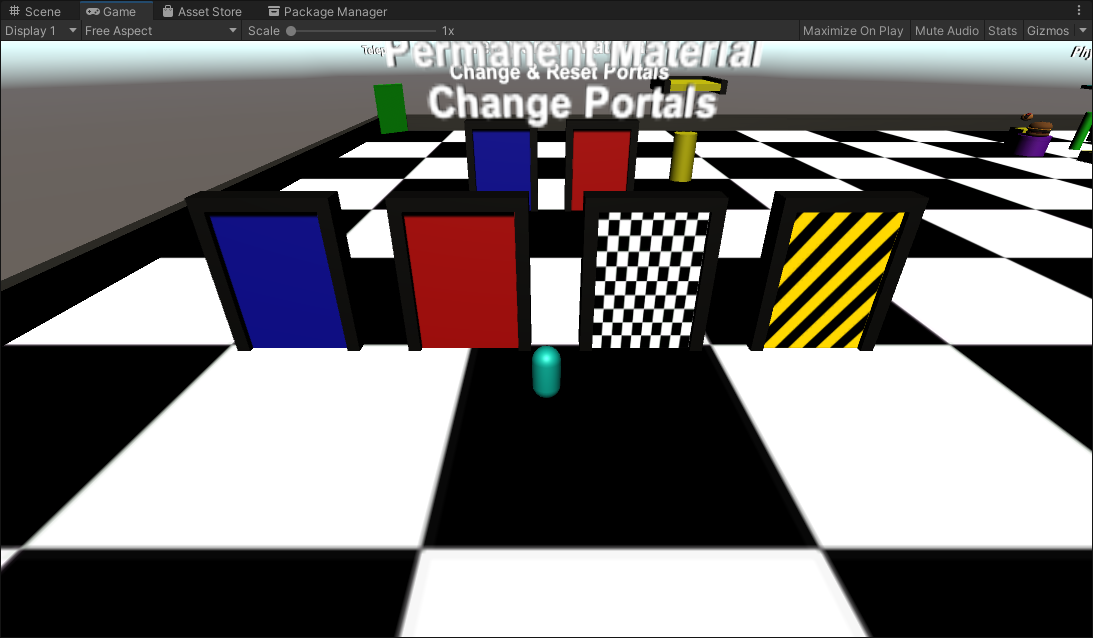
\includegraphics[width=.95\linewidth]{gfx/imgs/chapter4/PortaleCambiaColore1.png}
      \caption{Prima di aver attraversato il portale.}
      \label{fig:portale-colore-1}
    \end{subfigure}
    \begin{subfigure}{.49\textwidth}
      \centering
      % include second image
      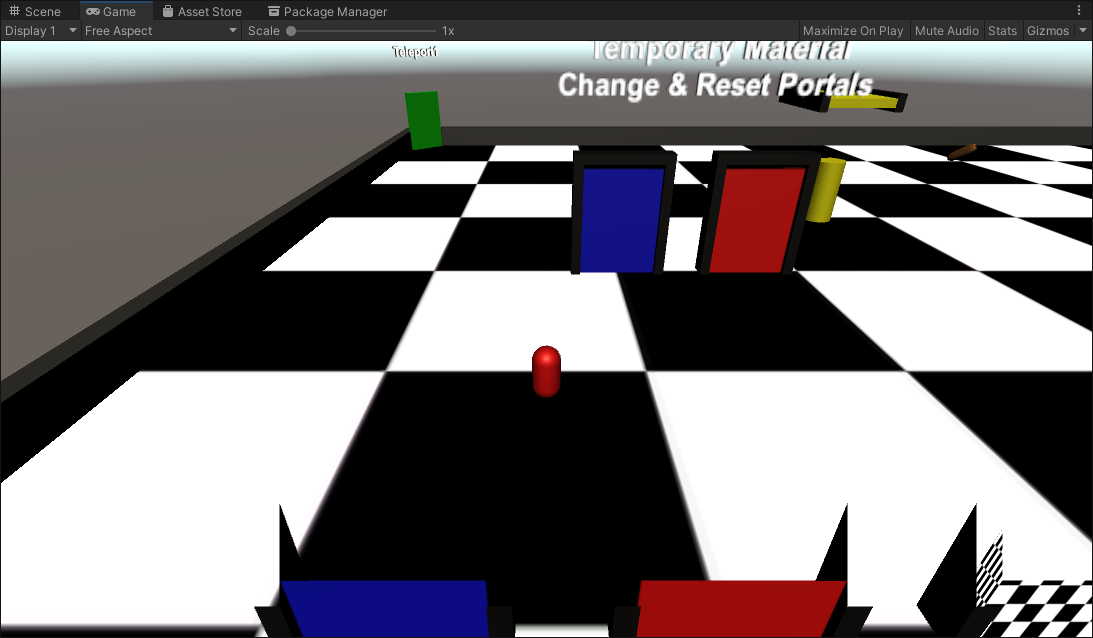
\includegraphics[width=.95\linewidth]{gfx/imgs/chapter4/PortaleCambiaColore2.png}
      \caption{Dopo aver attraversato il portale.}
      \label{fig:portale-colore-2}
    \end{subfigure}
    \caption{Portali cambia-colore (passaggio attraverso il portale rosso).}
    \label{fig:portali-cambia-colore}
\end{figure}

\subsubsection{Camera Follow}
Per rendere l'utilizzo del prototipo più piacevole ed evitare confusione con le varie capsule, abbiamo implementato un meccanismo che permette di ottenere una visuale in terza persona sulla propria entità \verb|CapsulePlayer|.

Il sistema \verb|CameraFollowPlayer| aggiorna la posizione della \verb|camera| principale, spostandola in base al componente \verb|Translation| dell'entità che possiede \verb|PlayerCameraFollowComponent|, ovvero la \verb|CapsulePlayer|. Per muovere solo la capsula del giocatore relativo, come per \verb|PlayerMovementSystem|, abbiamo utilizzato il singleton \verb|CommandTargetComponent|.

\begin{lstlisting}[caption={Componente che permette alla camera di seguire la capsula.}, label={lst:prototipo-camera-follow-component}, language={[Sharp]C}]
[GenerateAuthoringComponent]
public struct PlayerCameraFollowComponent : IComponentData
{
    public float xOffset;
    public float yOffset;
    public float zOffset;
}
\end{lstlisting}

\SaveVerb{CameraFollowPlayerTerm}|CameraFollowPlayer.cs|

\begin{lstlisting}[caption={File \UseVerb{CameraFollowPlayerTerm}: aggiornamento della posizione della camera per seguire la capsula del client.}, label={lst:prototipo-camera-follow-system}, language={[Sharp]C}]
[UpdateInGroup(typeof(ClientSimulationSystemGroup))]
public class CameraFollowPlayer : SystemBase
{
    protected override void OnUpdate()
    {
        var position = Camera.main.transform.position;

        var commandTargetComponentEntity =
            GetSingletonEntity<CommandTargetComponent>();
        var commandTargetComponent =
            GetComponent<CommandTargetComponent>(commandTargetComponentEntity);

        Entities
            .WithAll<PlayerScoreComponent>()
            .ForEach((Entity entity,
                in Translation translation, in PlayerCameraFollowComponent pcf) =>
        {
            // aggiorna solo la posizione rispetto alla propria capsula
            if (entity == commandTargetComponent.targetEntity)
            {
                position.x = translation.Value.x + pcf.xOffset;
                position.y = translation.Value.y + pcf.yOffset;
                position.z = translation.Value.z + pcf.zOffset;
            }
        }).Run();

        Camera.main.transform.position = position;
    }
}
\end{lstlisting}

\subsection{Build standalone}
Ai fini di testing della tesi abbiamo realizzato una sola build standalone per Windows, utilizzando il package \emph{Platforms Windows}. L'applicativo ci permette di eseguire il gioco come client, per cui è necessario avviare anche il server dall'editor Unity per poterlo utilizzare.

\begin{figure}[!ht]
    \begin{subfigure}{.49\textwidth}
      \centering
      % include first image
      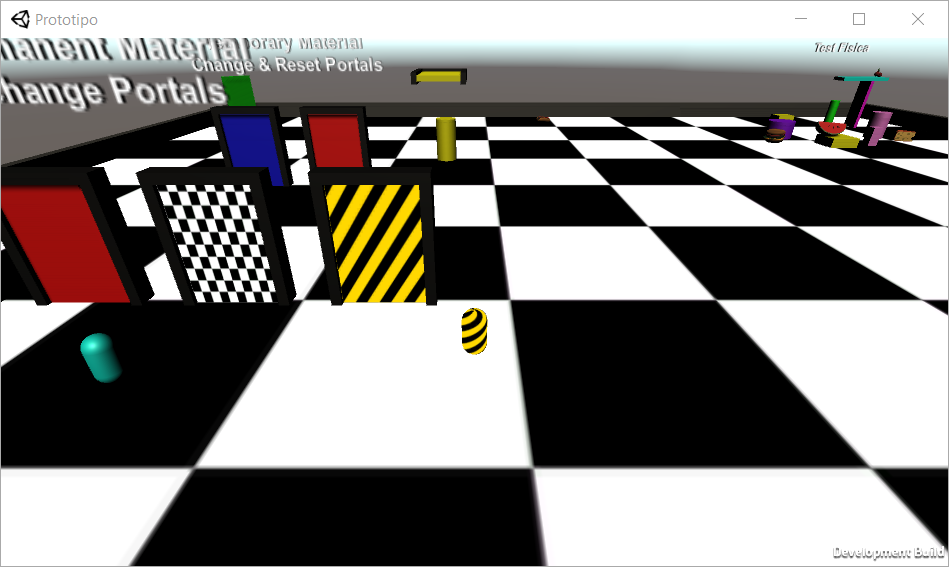
\includegraphics[width=.95\linewidth]{gfx/imgs/chapter4/BuildStandalonePrototipo.png}
      \caption{Build standalone (client).}
      \label{fig:build-standalone}
    \end{subfigure}
    \begin{subfigure}{.49\textwidth}
      \centering
      % include second image
      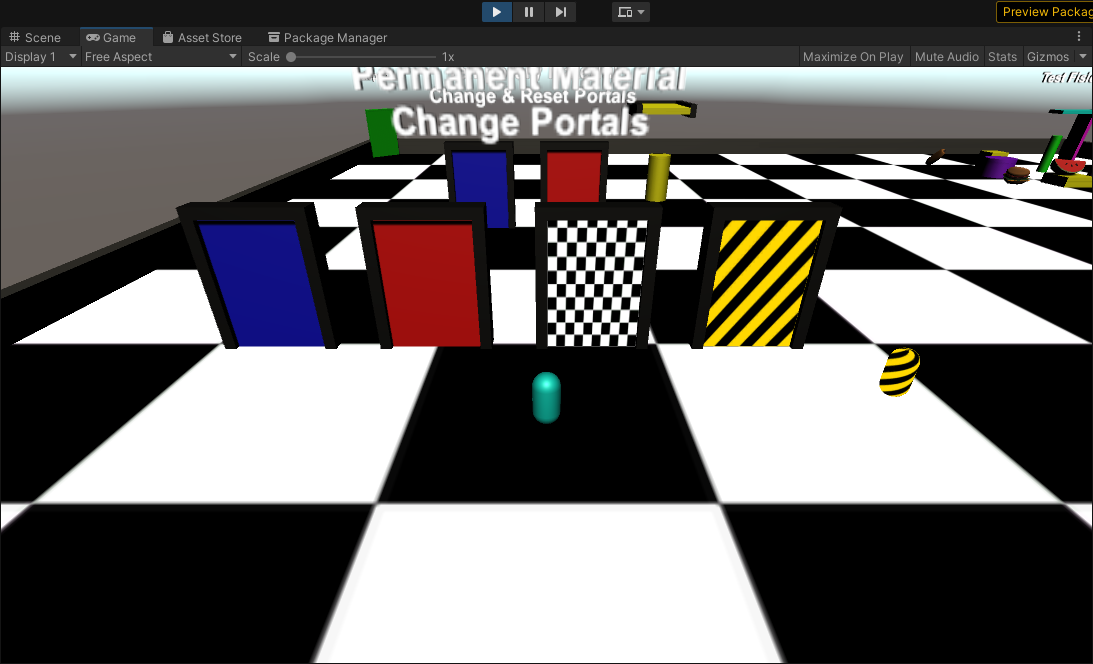
\includegraphics[width=.95\linewidth]{gfx/imgs/chapter4/BuildStandaloneEditor.png}
      \caption{Editor Unity (client \& server).}
      \label{fig:build-editor}
    \end{subfigure}
    \caption{Avvio da Unity in modalità ``Client \& Server'' e connessione dall'applicativo client standalone.}
    \label{fig:build}
\end{figure}
